\chapter{Introducción}

En este capítulo no deben faltar los siguientes apartados:

\section{Motivación del proyecto}

En los últimos años el consumo de energía primaria en España ha aumentado significativamente de unos 88455 ktep($\sim1.03E12 \ kWh$) en 1990 a unos 126107 ktep($\sim 1.43E12 \ kWh$) en 2019, que equivale a un aumento del 42\% respecto a su valor en 1990, llegando a ser su valor máximo unos 146891 ktep($\sim 1.71E12 \ kWh$) en 2007.\\\\
De 2008 a 2014, como consecuencia de la crisis económica el consumo energético disminuyó hasta unos 117824 ktep ($\sim 1.37E12 \ kWh$) en 2014, recuperándose a partir del 2015, como se puede observar en la figura \ref{fig:demandaenergiaprimariaproporcion1990}. \\


\begin{figure}[H]
	\centering
	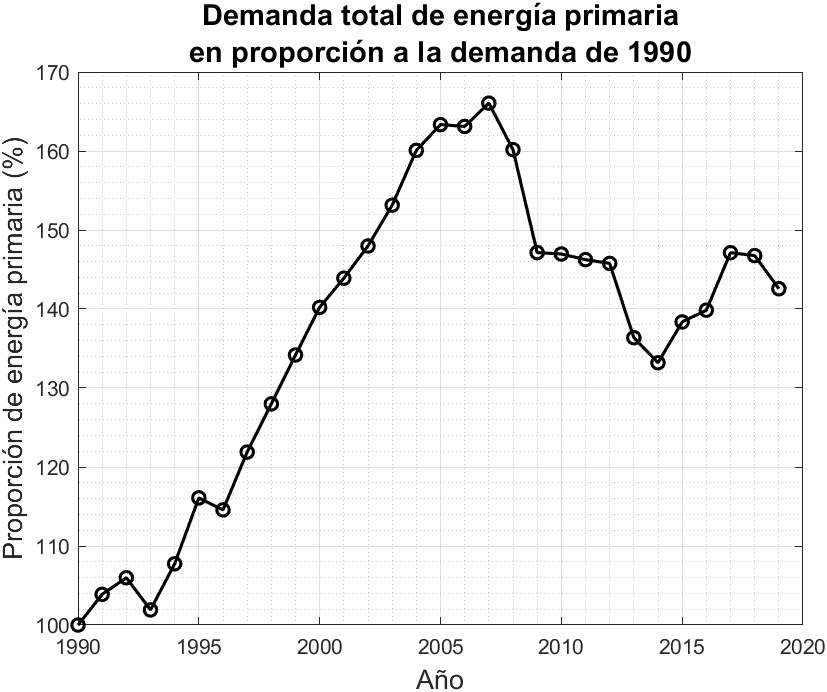
\includegraphics[width=10cm, height=7cm]{figuras/DemandaEnergiaPrimariaProporcion1990}
	\caption[Relación entre demanda total de energía primaria anual]{Representación gráfica de la relación entre la demanda total de energía primaria anual de 1990 hasta 2019 en España. \textit{Fuente obtención de datos: Ministerio para la transición ecológica y el reto demográfico de España.} }
	\label{fig:demandaenergiaprimariaproporcion1990}
\end{figure}
Dicha energía se puede dividir en diferentes categorías según el sector que la consume o la fuente de dicha energía. En el 2019, un 44.5\% de la energía primaria fue consumida de productos petrolíferos y apenas un 14.5\% de renovables (figura \ref{fig:fuentesenergiasprimarias}), y un 23.6\% de la energía final fue consumida por el sector de la industria (figura \ref{fig:consumoenergiafinalporsectores2019}), representando casi una cuarta parte del consumo total de la energía final en España. Des-afortunadamente la energía consumida no es completamente aprovechada, llamada calor residual. En 2015, la industria en España consumió aproximadamente 220 TWh de energía, desperdiciándose unos 22 TWh según los cálculos de las estimaciones realizadas en \cite{wasteEnergyindustryEstimate}.

\begin{figure}[H]
	\centering
	\begin{subfigure}[b]{0.48\textwidth}
		\includegraphics[width=\textwidth]{figuras/FuentesEnergíasPrimarias}
		\caption{Consumo de energía por fuente}
		\label{fig:fuentesenergiasprimarias}
	\end{subfigure}
	\hfill
	\begin{subfigure}[b]{0.48\textwidth}
		\centering
		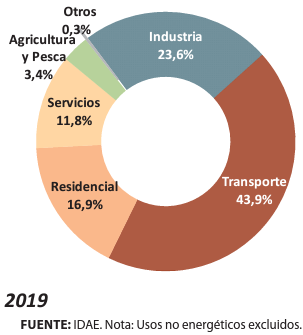
\includegraphics[width=\textwidth]{figuras/consumoEnergiaFinalPorSectores_2019}
		\caption{Consumo de energía por sectores.}
		\label{fig:consumoenergiafinalporsectores2019}
	\end{subfigure}
\caption[]{Desglose del consumo de energía primaria en España 2019 por fuente de energía(\subref{fig:fuentesenergiasprimarias}). Consumo de energía final por sectores en el año 2019 en España(\subref{fig:consumoenergiafinalporsectores2019}). \textit{Fuente:  Ministerio para la transición ecológica y el reto demográfico de España.} }
 \label{fig:consumosEnergiasCategorias}
\end{figure}

Para recuperar esta energía perdida se han desarrollado instalaciones de recuperación de calor residual, no solo para disminuir los costes sino también para disminuir las emisiones de contaminantes, cumpliendo así parte de los objetivos de desarrollo sostenible. Estas instalaciones o sistemas no se limitan exclusivamente al sector industrial, por ejemplo, en el sector residencial se utilizan sistemas fotovoltaicos con un sistema de enfriamiento que permite enfriar las células y calentar el agua para su posterior uso.\\ 

El calor residual se puede aprovechar para obtener electricidad o para calentar un fluido para mejorar la eficiencia del mismo u otro proceso, disminuyendo el consumo de combustible u energía. El uso del calor residual para el calentamiento de otro fluido para su utilización se usa en la industria con un dispositivo llamado economizador que se usa en calderas, mejorando el rendimiento térmico. La obtención de electricidad mediante el aprovechamiento del calor residual puede ser por vía de trabajo mecánico o por conversión directa.

La conversión  se da por ciclos termodinámicos, principalmente el de Rankine, donde se intercambia calor con agua, formándose vapor que luego hace mover una turbina que está conectada a un generador.\\

Un ejemplo de un sistema de aprovechamiento del calor residual de un proceso es la co-generación que aprovecha el calor sobrante de la conversión termo-eléctrica y los ciclos combinados que aprovechan el calor residual de la turbina de gas para ebullir agua y alimentar una turbina de vapor.\\

 Otro ejemplo del aprovechamiento del calor residual por el ciclo de Rankine es la  planta de valorización energética del Centro Las Lomas del Parque Tecnológico de Valdemingómez que trata los residuos de rechazos de tratamiento y otros residuos urbanos no aprovechables o de difícil tratamiento que son incinerados en un horno y cuyos gases son enfriados en una caldera, aprovechando el calor para obtener electricidad, para luego seguir con su tratamiento (figura \ref{fig:esquemaslomasvalorizacion}).\\
\begin{figure}[H]
	\centering
	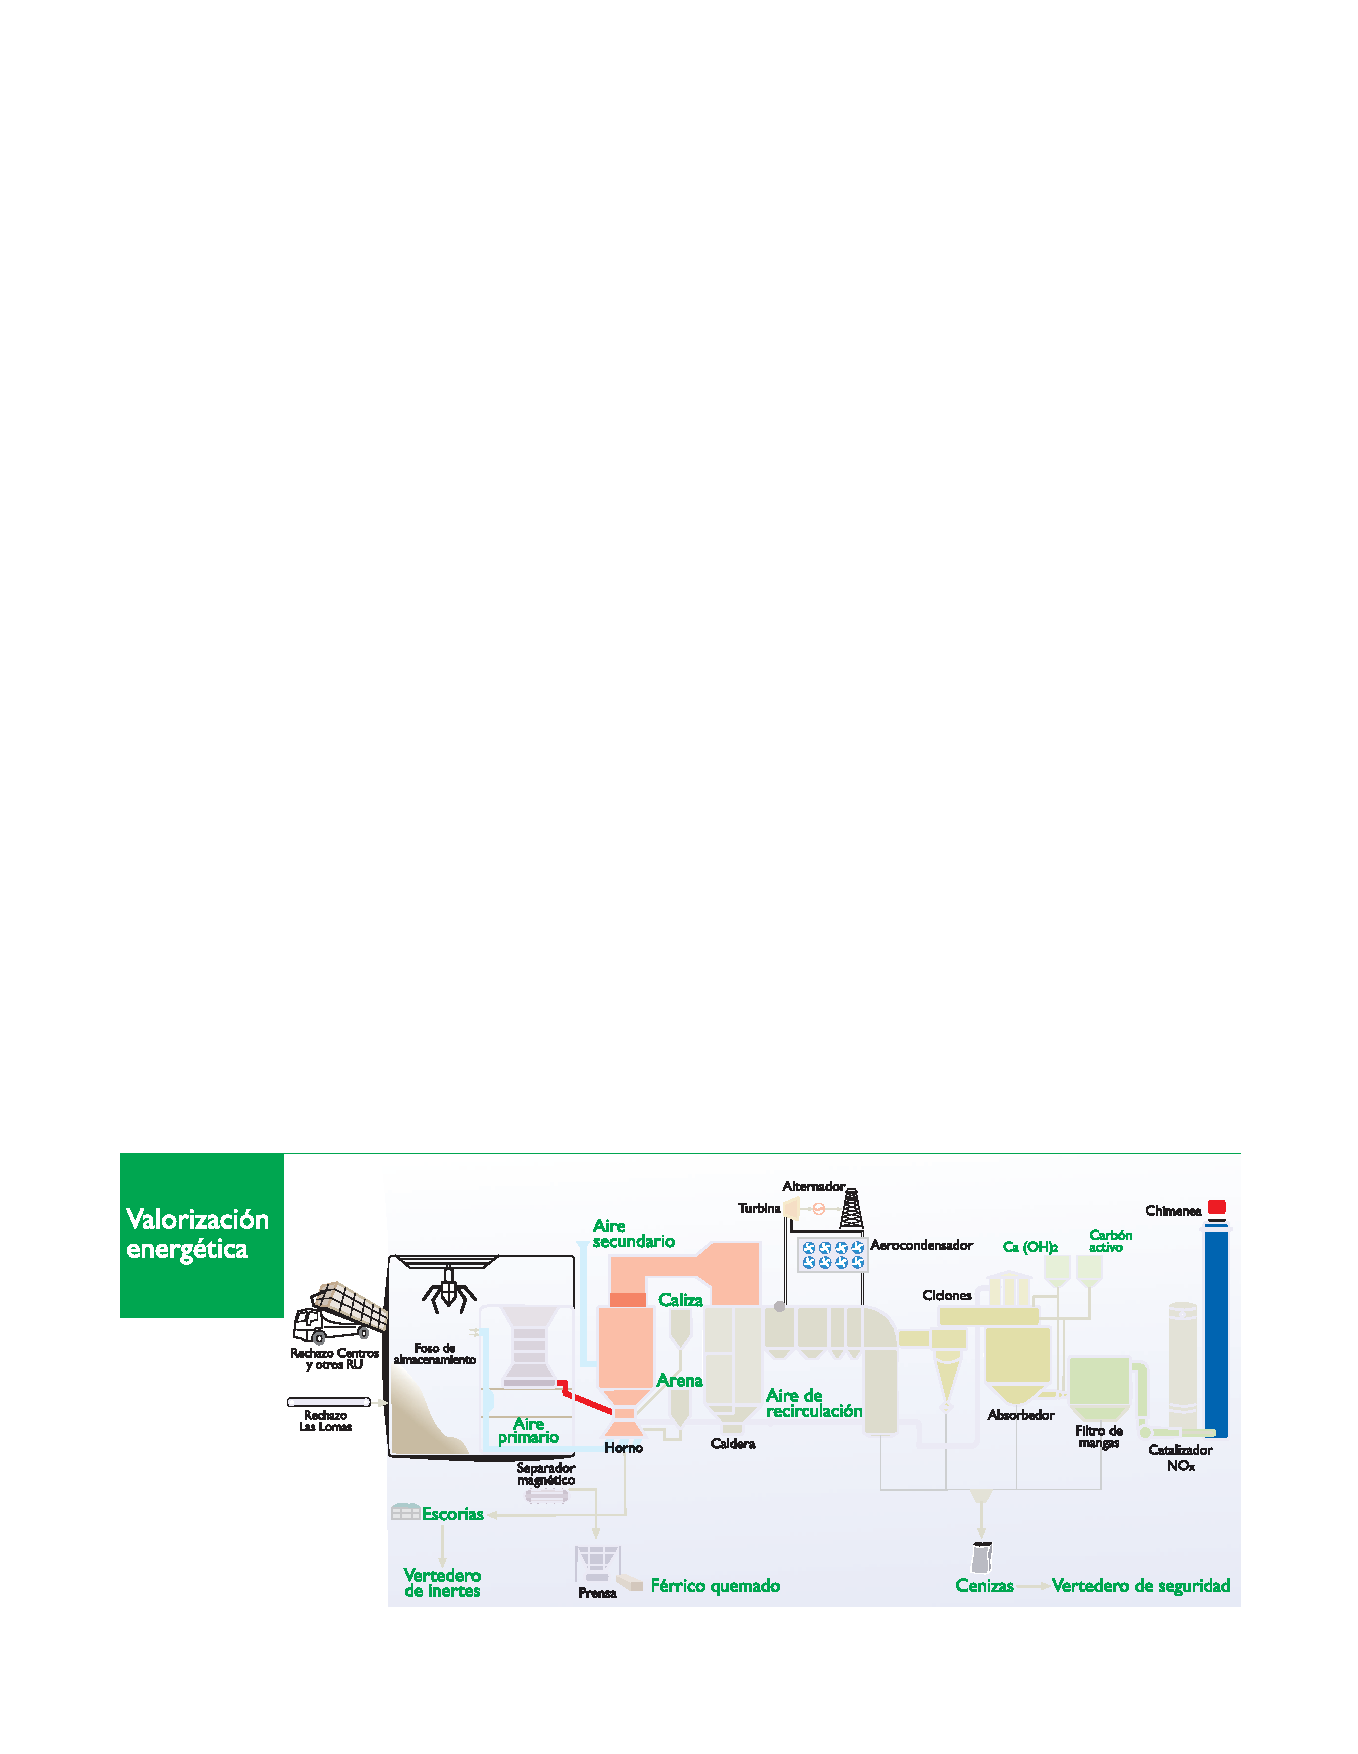
\includegraphics[height=5cm]{figuras/esquemasLomasValorizacion}
	\caption{Planta de valorización energética del Centro Las Lomas del Parque Tecnológico de Valdemingómez. \textit{Fuente: Ayuntamiento de Madrid}}
	\label{fig:esquemaslomasvalorizacion}
\end{figure}

El problema principal con un sistema de este tipo son las partes móviles, las cuales tienen que estar en constante mantenimiento, para disminuir el mantenimiento se puede pasar a un sistema de recuperación de calor residual que no tenga partes móviles, una forma de recuperar el calor es mediante un sistema termo-fotovoltaico que aprovecha la radiación que emite un cuerpo para transformarlo en electricidad en corriente continua.




  año en el cual la ONU (Organización de las Naciones Unidas) aprobó la \textit{Agenda 2030 sobre el Desarrollo Sostenible}, la cual cuenta con 17 objetivos de desarrollo sostenible (ODS)

\textbf{De energías por fuente->energías por sector-> Artículo de internet -> TPVs->Motivación del proyecto}

\begin{figure}[H]
	\centering
	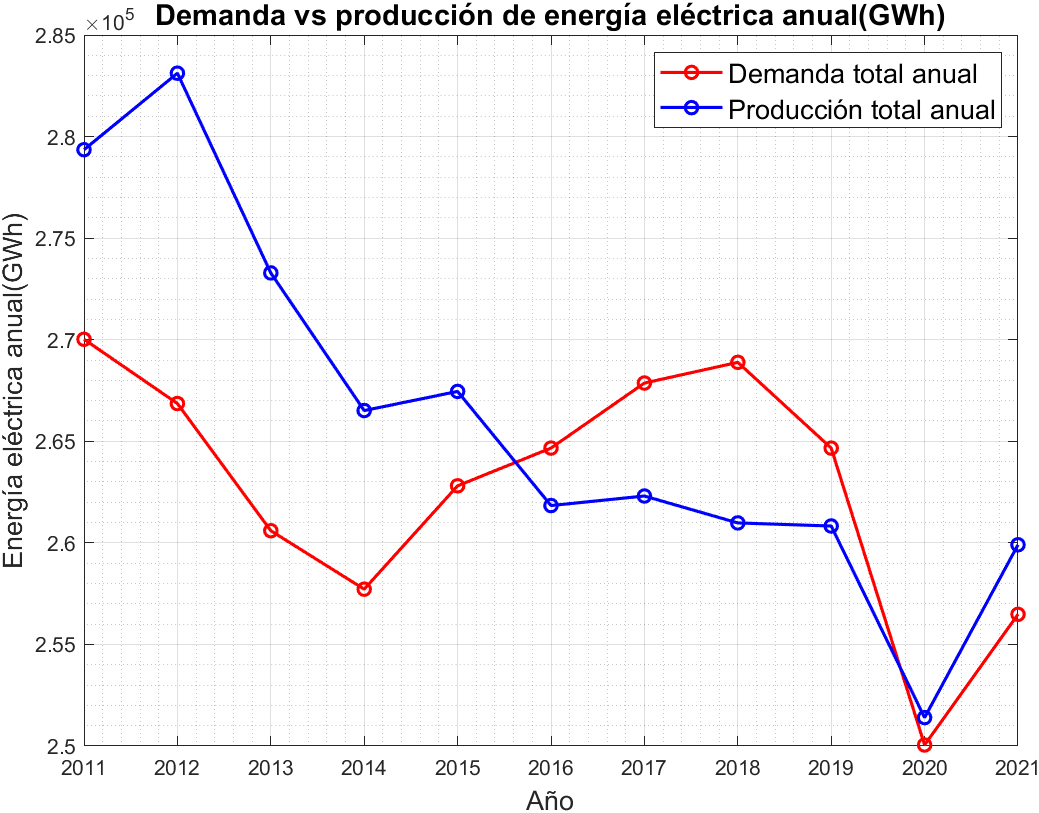
\includegraphics[width=10cm, height=7cm]{figuras/ProdcVSdemAnual}
	\caption[Producción vs demanda de energía eléctrica anual]{Comparación de la producción vs la demanda de energía eléctrica anual de España entre los años 2011 y 2021. \textit{Fuente: red eléctrica de España.} }
	\label{fig:prodcvsdemanual}
\end{figure}

\begin{figure}[h]

\end{figure}


% Aquí irá el gran cantidad de energía que se desperdicia en las fábricas, refinerías, etc.
% Así como se puede aprovechar mediante la termo-fotovoltaíca.



\section{Objetivos}
El objetivo de este estudio es diseñar y simular pilares de dimensiones nanométricas para el aprovechamiento del efecto de campo cercano en un convertidor termo-fotovoltaico, así como determinar la viabilidad de este sistema. 
\begin{itemize}
	\item Modelar un nano-espaciador dentro de los rangos permitidos de los parámetros de los programas de simulación y modelado 3D.
	\item Modelar el emisor y la célula del sistema TPV para que los gradientes térmicos por conducción no lleguen a los bordes.
	\item Simular la transferencia de calor por conducción a través de un nano-espaciador de $SiO_2$ de un sistema TPV para diferentes alturas del nano-espaciador, diferentes materiales de emisor y diferentes resistencias de contacto entre emisor y el nano-espaciador.
	\item Simular la transferencia de calor radiada entre el emisor y la célula para diferentes materiales del emisor y para varias distancias de separación, teniendo en cuenta los efectos de campo cercano en la radiación.
	\item Determinar entre los casos estudiados cuales pueden dar lugar a sistemas de TPV de campo cercano viables.
\end{itemize}


\section{Estructura del documento}

A continuación y para facilitar la lectura del documento, se detalla el contenido de cada capítulo.

\begin{itemize}
\item En el \textbf{capítulo 1} se realiza una introducción del trabajo con la respectiva motivación y objetivos.
\item En el \textbf{capítulo 2} se desarrolla el estado de arte, definiendo los apartados más importantes y resaltando las investigaciones con mayor relevancia.
\item En el \textbf{capítulo 3} se exponen las herramientas y materiales utilizados, así como los criterios de selección.
\item En el \textbf{capítulo 4} se mencionan los métodos seguidos y los cálculos realizados para el desarrollo del trabajo.
\item En el \textbf{capítulo 5} se exponen los resultados obtenidos de las simulaciones.
\item En el \textbf{capítulo 6} se desarrolla la conclusión y se realiza planteamientos para futuros trabajos.
\end{itemize}
